\documentclass[a4paper]{article}
\usepackage[left=2.1cm, right=2.1cm, top=2.1cm]{geometry}
\usepackage{lipsum}
\usepackage{tikzpagenodes}
\usepackage{pgfplots}
\usepackage{tikz}
\usepackage{tikz-3dplot}
\usetikzlibrary{arrows,decorations.pathmorphing,backgrounds,positioning,fit,matrix}
\pgfplotsset{compat=1.8}
\usepackage{graphics} % for pdf, bitmapped graphics files
\usepackage{epsfig} % for postscript graphics files
\usepackage[colorlinks=true,citecolor=green]{hyperref}
\usepackage{cite}
\usepackage{amsmath,amssymb,amsfonts}
\usepackage{algorithmic}
\usepackage{graphicx}
\usepackage{url}
\usepackage{cite}
\usepackage{bm}
\usepackage{pbox}
\usepackage{siunitx,booktabs,etoolbox}
\usepackage{ulem}
\usepackage[framed,numbered,autolinebreaks,useliterate]{mcode}
\usepackage{filecontents}
%\usepackage{bigfoot} % to allow verbatim in footnote


\def\BibTeX{{\rm B\kern-.05em{\sc i\kern-.025em b}\kern-.08em
    T\kern-.1667em\lower.7ex\hbox{E}\kern-.125emX}}
\begin{filecontents*}{box.m}
clear
close all
Q=Box3D;
plot3(Q(1,:),Q(2,:),Q(3,:),'.'),
axis equal
axis([-1 1 -1 1 -1 5])
xlabel('x')
ylabel('y')
zlabel('z')
\end{filecontents*}
\begin{filecontents*}{cube.m}
x = 0:0.1:5;
y = 0:0.1:5;
pt = [x repmat(x(end), 1, numel(y)) fliplr(x) repmat(x(1), 1, numel(y)); repmat(y(1), 1, numel(y)) y repmat(y(end), 1, numel(y)) fliplr(y)];
pt = [pt;ones(1,size(pt,2))];  
\end{filecontents*}

\begin{filecontents*}{fdata.m}
	%% loading
    im1 = rgb2gray(imread('000002.bmp'));
    im2 = rgb2gray(imread('000003.bmp'));
    load('calib.mat');
    [im1,~] = undistortImage(im1,cameraParams);
    [im2,~] = undistortImage(im2,cameraParams);
   	
   	load('Fdata.mat');

    im3 = cat(2,im1,im2);
    figure;imshow(im3);hold on;

    plot(x1(:,1),x1(:,2),'ro');
    plot(x2(:,1)+size(im1,2),x2(:,2),'go');

    shift = size(im1,2);
    cmap = lines(5);
    k = 1;
    for i = 1:size(x1,1)
	    ptdraw = [x1(i,1), x1(i,2);
                  x2(i,1)+shift, x2(i,2)];
        plot(ptdraw(:,1),ptdraw(:,2),'LineStyle','-','LineWidth',1,'Color',cmap(k,:));
        k = mod(k+1,5);if k == 0 k = 1;end
    end
    
	%% here starts your code, 
    F = DLT8pt(x1',x2');
	
	%% once you have estimated F, check your F using
    vgg_gui_F(im1,im2,F');
    
\end{filecontents*}

\begin{filecontents*}{tri1.m}
    N = 100;
    p = rand([3,N]) * 10 - 5;% from near to far
    p(1,:) = p(1,:) + 15;
    C1 = [0;0;0];
    C2 = [0;0.2;0];

    rad1 = -10/57.3;
    R1 = [cos(rad1) 0 -sin(rad1);0 1 0;sin(rad1) 0 cos(rad1)]*[0 -1 0;0 0 -1;1 0 0];
    R2 = [cos(-rad1) 0 -sin(-rad1);0 1 0;sin(-rad1) 0 cos(-rad1)]*[0 -1 0;0 0 -1;1 0 0];

    t1 = -R1*C1;
    t2 = -R2*C2;

    figure
    h1 = plot3(p(1,:),p(2,:),p(3,:),'g*');hold on;
    cam1 = plotCamera('Location',C1,'Orientation',R1,'Opacity',0,'Color',[1 0 0],'Size',0.4,'Label','Camera1');
    cam2 = plotCamera('Location',C2,'Orientation',R2,'Opacity',0,'Color',[0 1 0],'Size',0.4,'Label','Camera2');
    axis equal
    xlabel('x:(m)');
    ylabel('y:(m)');
    zlabel('z:(m)');
    title('Triangulation Simulation');
    set(gca,'FontName','Arial','FontSize',20);

    K = [500 0 320;0 500 240;0 0 1];

    [uv1, in1] = proj(R1,t1, p, K);
    [uv2, in2] = proj(R2,t2, p, K);

    in = in1 & in2;
    q1 = uv1(:,in);
    ptrue = p(:,in);
    q2 = uv2(:,in);

    q1(1:2,:) = q1(1:2,:);
    q2(1:2,:) = q2(1:2,:);

    P1 = K*[R1 t1];
    P2 = K*[R2 t2];
    
    precons = zeros(3,size(q1,2));
    for i = 1:size(q1,2)
    	%% here starts your code
        precons(:,i) = triangulation(q1(:,i),P1,q2(:,i),P2);
    end
    
    %% visualization
    figure
    plot3(ptrue(1,:),ptrue(2,:),ptrue(3,:),'ro','MarkerSize',8);hold on;
    plot3(precons(1,:),precons(2,:),precons(3,:),'g+','MarkerSize',8);hold on;
    xlabel('x:(m)');
    ylabel('y:(m)');
    zlabel('z:(m)');
    title('Triangulation Simulation');
    legend({'Truth','Reconstruction'});
    set(gca,'FontName','Arial','FontSize',20);
    grid on;    
    
\end{filecontents*}


\begin{filecontents*}{tri2.m}
    baseDir = './images/';% use you own directory
    buildingScene = imageDatastore(baseDir);
    numImages = numel(buildingScene.Files);

    load(strcat(baseDir,'viff.xy'));
    x = viff(1:end,1:2:72)';  % pull out x coord of all tracks
    y = viff(1:end,2:2:72)';  % pull out y coord of all tracks

	% visualization
    num = 0;
    for n = 1:numImages-1
        im1 = readimage(buildingScene, n);
        imshow(im1); hold on;
        id = x(n,:) ~= -1 & y(n,:) ~= -1;
        plot(x(n,id),y(n,id),'go'); 
        num = num + sum(id);
        hold off;
        pause(0.1);
    end

	% load projection matrices
    load(strcat(baseDir,'dino_Ps.mat'));


    ptcloud = zeros(3,num);
    k = 1;
    for i = 1:size(x,1)-1
        % tracked features
        id = x(i,:) ~= -1 & y(i,:) ~= -1 & x(i+1,:) ~= -1 & y(i+1,:) ~= -1;
        q1 = [x(i,id);y(i,id);];
        q2 = [x(i+1,id);y(i+1,id);];
		P1 = P{i};
        P2 = P{i+1};        
        
        precons = zeros(3,size(q1,2));
        for j = 1:size(q1,2)
            % your code starts
            precons(:,j) = xxxxx(q1(:,j),P1,q2(:,j),P2);
        end        
		
        ptcloud(:,k:k+size(q1,2)-1) = precons;
        k = k + size(q1,2);
    end
    figure
    plot3(ptcloud(1,:),ptcloud(2,:),ptcloud(3,:),'k.','MarkerSize',10);hold on;
    grid on;
    axis equal;
    view(3);
    for i = 1:size(x,1)
        P1 = P{i};
        [K, R, t, c] = decomposeP(P1);
        plotCamera('Location',c,'Orientation',R,'Opacity',0,'Color',[0 1 0],'Size',0.05);
    end

\end{filecontents*}


\begin{filecontents*}{tri3.m}
    I1 = imread('im0.png');
    I2 = imread('im1.png');
    figure;imshow(I1);
    
    load('disp.mat');
    disparityRange = [0 480];
    figure
    imshow(disparityMap,disparityRange)
    title('Disparity Map')
    colormap jet
    colorbar
    % stereo vision intrinsics
    f = 4841.191;
    px = 1441.607;
    py = 969.311;
    % baseline: m
    b = 170.458*1e-3;
    % only triangulate pixel whose disparity is within [100,480].
    id = disparityMap >= 100 & disparityMap <= 480;
    
    % your code starts
    ptcloud = xxxx(disparityMap, f, px, py, b, id);
    
    % display point cloud
    colorcloud = uint8(zeros(size(ptcloud,1),3));
    r = I1(:,:,1); g = I1(:,:,2); b = I1(:,:,3);
    colorcloud(:,1) = r(id);
    colorcloud(:,2) = g(id);
    colorcloud(:,3) = b(id);
    ptCloud = pointCloud(ptcloud,'Color',colorcloud);
    pcshow(ptCloud);
\end{filecontents*}


\begin{document}

\title{Exercise on Epipolar Geometry \& Triangulation}
%\author{xiahaa@space.dtu.dk}
\maketitle%%

In this exercise, we will work with a few assignments related to epipolar geometry and triangulation.

\section{Epipolar Geometry}
In this exercise, you will work on fundamental matrix estimation using the famous Eight-point algorithm. Recall the epipolar constraint formed with the fundamental matrix as
$$
\mathbf{x}_2^T\mathbf{F}\mathbf{x}_1=0
$$
where $\mathbf{x}_1=[x_1,y_1,1]^T$ (homogeneous coordinate) denotes the point in image $1$ with its corresponding point in image $2$ being $\mathbf{x}_2=[x_2,y_2,1]^T$, $\mathbf{F}$ is the fundamental matrix. Expanding this equation, we will have the following linear equation:
\begin{align*}
[x_2,y_2,1]\left[\begin{matrix}
f_{11} & f_{12} & f_{13} \\
f_{21} & f_{22} & f_{23} \\
f_{31} & f_{32} & f_{33} 
\end{matrix}\right]\left[\begin{matrix}
x_1 \\
y_1 \\
1
\end{matrix}\right]=0 \Rightarrow \\
\left[\begin{matrix}
x_1x_2 & x_1y_2 & x_1 & y_1x_2 & y_1y_2 & y_1 & x_2 & y_2 & 1
\end{matrix}\right]\left[\begin{matrix}
f_{11} \\
f_{21} \\
f_{31} \\
f_{12} \\
f_{22} \\
f_{32} \\
f_{13} \\
f_{23} \\
f_{33} 
\end{matrix}\right]=0
\end{align*}
We need at least $8$ points to determine $\mathbf{F}$\footnote{$\mathbf{F}$ is determined up to a scale, so without losing generality, we can make $f_{33}=1$ and then there are $8$ unknowns left.}. Stacking them together will give us a linear system:
$$
\mathbf{Ax}=0
$$
where $\mathbf{x}=[f_{11}, f_{21}, f_{31}, f_{12}, f_{22},f_{32},f_{13},f_{23},f_{33}]^T$.
By solving $\mathbf{x}$ using SVD, the fundamental matrix can be estimated.
\begin{figure*}[!b]
\centering
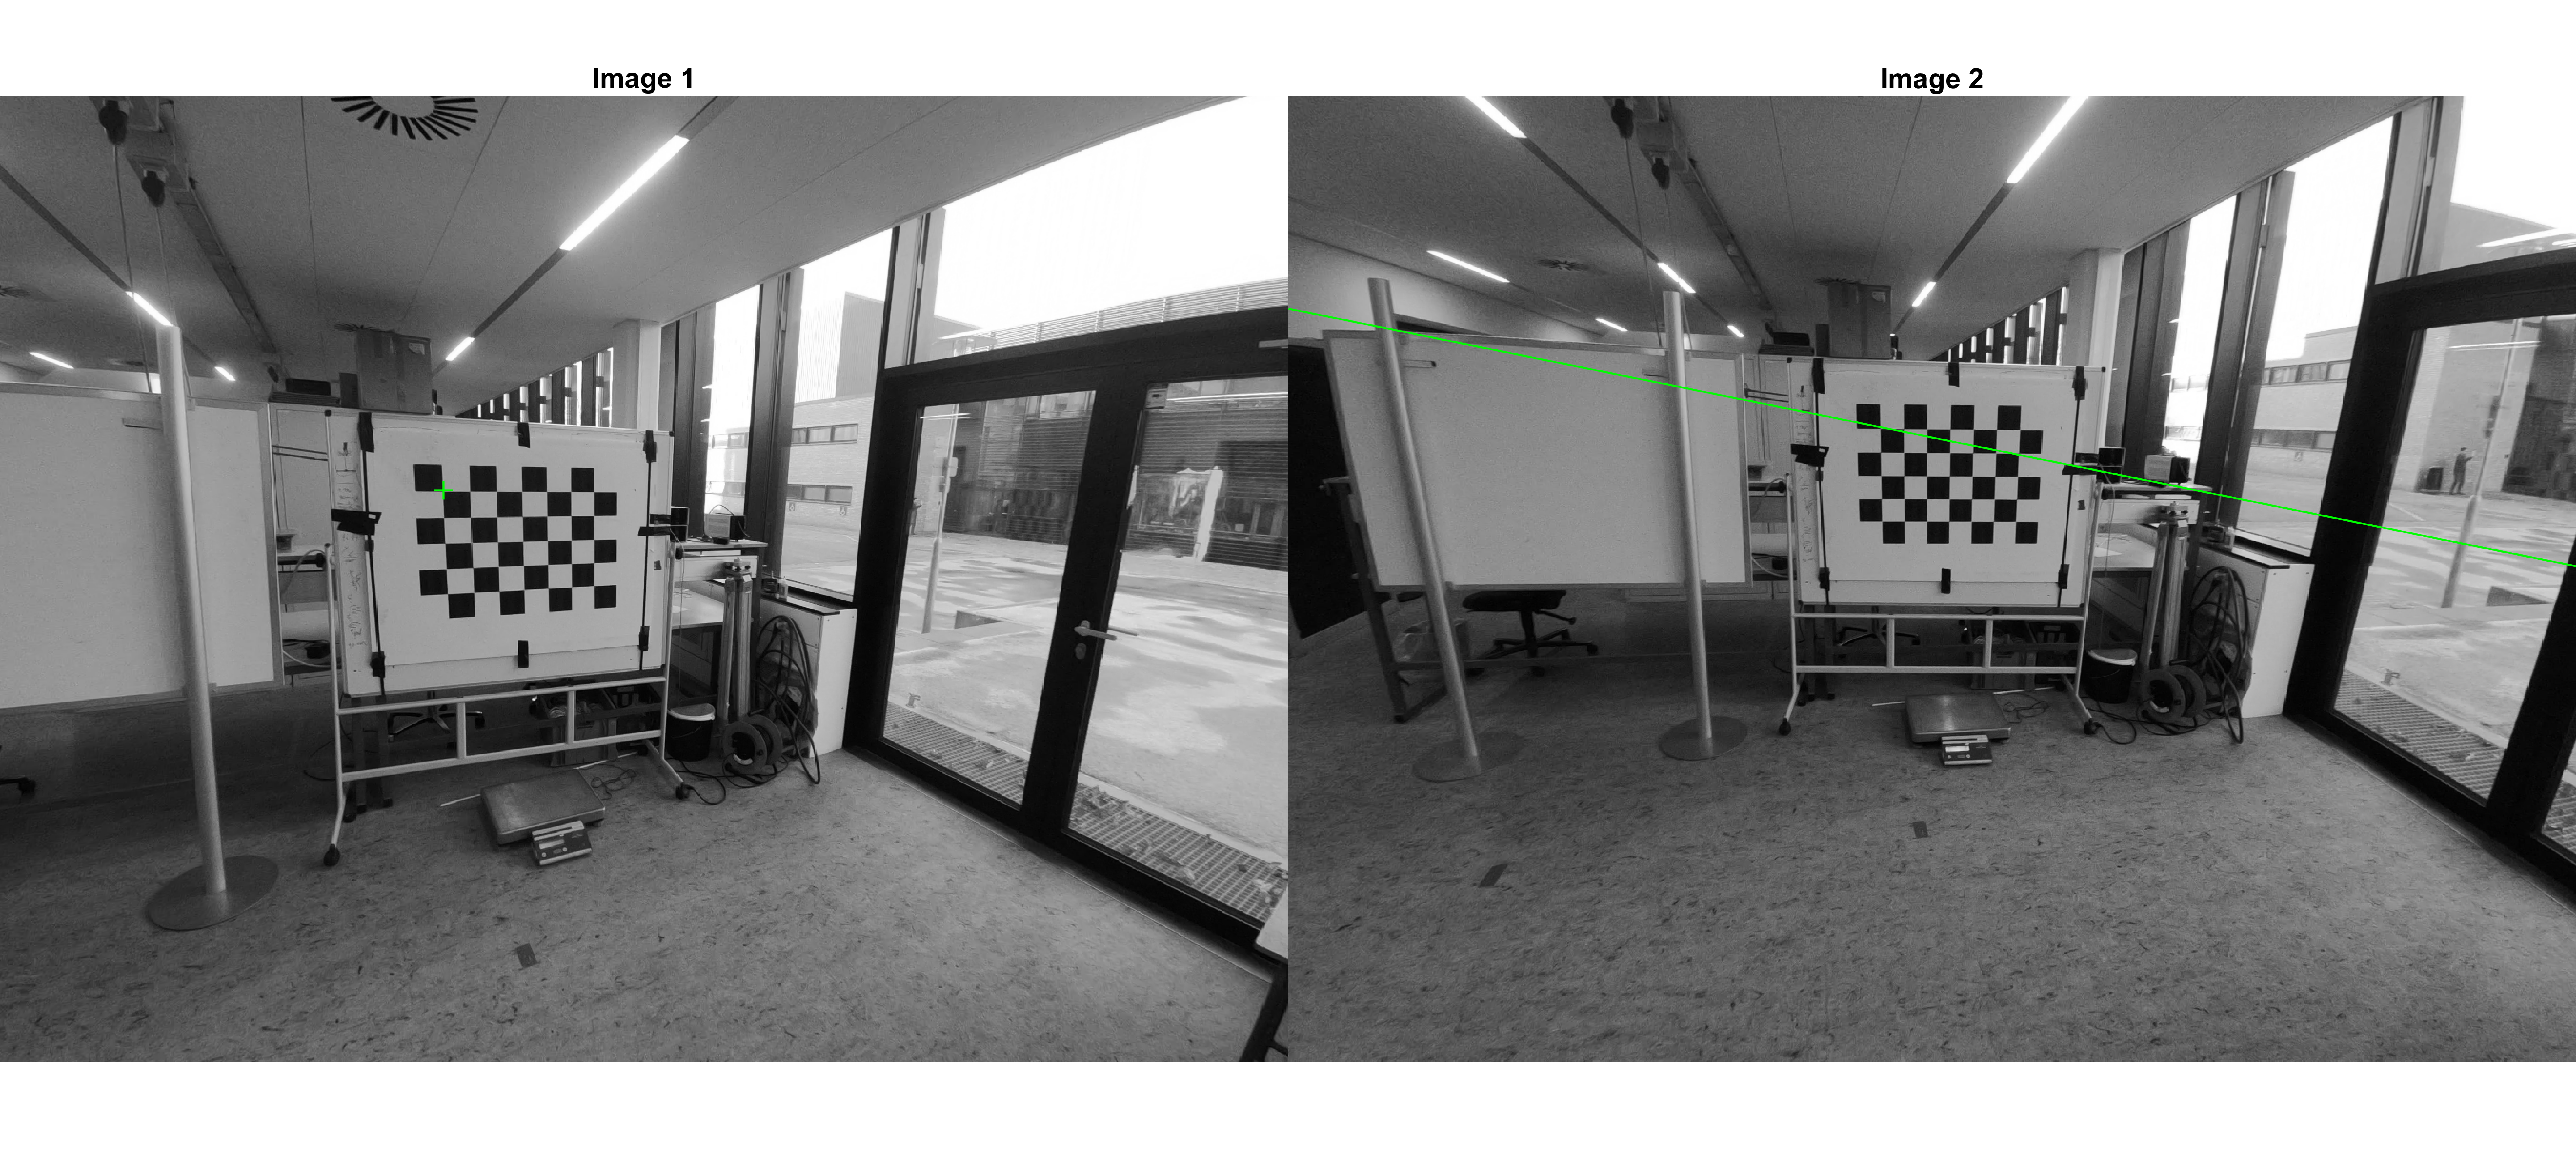
\includegraphics[scale=0.3]{figures/f.png}
\caption{Check you result visually using epipolar geometry. If the $\mathbf{F}$ is accurately estimated, then by for one point (green $+$) in image $1$, its corresponding point in image $2$ will be on the epipolar line (green line).}
\end{figure*}
\paragraph{Q1:} 
Implement the Eight-point algorithm use the provided data (\textbf{Fdata.mat}) as the input. \textbf{Fdata.mat} contains feature points detected and matched. You can visualize using the following code:
\lstinputlisting{fdata.m}
\paragraph{Q2:} 
Once you have estimate $\mathbf{F}$, you can check your result visually. 

\section{Triangulation}
In this exercise, you need to implement the triangulation method (\textcolor{blue}{the SVD approach}) you have learnt from the lecture. You start with simulated data and then work with real images.
\paragraph{Q3:} 
Use the following code to generate simulated data for triangulation
\lstinputlisting{tri1.m}

\paragraph{Q4:} 
Now you will apply your triangulation code on real images\footnote{Data source: "Dinosaur" from \url{www.robots.ox.ac.uk/~vgg/data/data-mview.html}.}. To save your time, parsing code is provided as follows:
\lstinputlisting{tri2.m}. If your implementation is correct, you will see a dinosaur.
\begin{figure*}[!b]
\centering
\includegraphics[scale=0.5]{figures/dino.png}
\caption{Dinosaur triangulated.}
\end{figure*}

\paragraph{Q5:}
Triangulation can be made much easily if stereo vision system is used. In this exercise, you will implement the triangulation method for stereo vision. Stereo images\footnote{Source: "Mask" from \url{vision.middlebury.edu/stereo/data/2014/}} and the corresponding disparity are provided. The following code is provided for data parsing and visualization.
\lstinputlisting{tri3.m}

The equations for triangulate points using disparity are given as:
\begin{align*}
Z &= \frac{f*b}{d} \\
X &= \frac{(x-p_x)Z}{f} \\ 
Y &= \frac{(y-p_y)Z}{f}
\end{align*}
here, $p_x,p_y$ are the coordinates of the principal point, $f$ is the focus length, $b$ is the baseline.

\textbf{Note: $p_x$ ($p_y$, resp) is given along the image width (height, resp) direction, while $(x,y)$ in \textsc{Matlab} corresponds to the point at $x^{th}$ row and $j^{th}$ column.} 

\begin{figure*}[!b]
\centering
\includegraphics[scale=0.5]{figures/stereo.png}
\caption{Result obtained by triangulating stereo images.}
\end{figure*}
 
\bibliography{hand_eye_calibration} 
\bibliographystyle{ieeetr}

\end{document}